\documentclass[xetex,mathserif,serif]{beamer}
\usepackage{polyglossia}
\setdefaultlanguage[babelshorthands=true]{russian}
\usepackage{minted}

\useoutertheme{infolines}

\setmainfont{FreeSans}
\newfontfamily{\russianfonttt}{FreeSans}

\definecolor{links}{HTML}{2A1B81}
\hypersetup{colorlinks,linkcolor=,urlcolor=links}

\title{Объектно-ориентированное программирование на C\#}
\subtitle{Введение}
\author[Юрий Литвинов]{Юрий Литвинов \newline \textcolor{gray}{\small\texttt{yurii.litvinov@gmail.com}}}
\date{14.02.2020г}

\begin{document}
	
	\frame{\titlepage}

	\section{Организационное}

	\begin{frame}
		\frametitle{Про что этот курс}
		\begin{itemize}
			\item Объектно-ориентированное программирование и близкие вещи
			\begin{itemize}
				\item Абстракция-инкапсуляция-наследование-полиморфизм
				\item Исключения
				\item Генерики
				\item События
				\item Пользовательские интерфейсы
			\end{itemize}
			\item Технология разработки ПО
			\begin{itemize}
				\item Юнит-тесты
				\item CI
				\item Визуальное моделирование
			\end{itemize}
			\item Язык --- C\#
			\item Не будет новых алгоритмов, будут новые технологии
		\end{itemize}
	\end{frame}

	\begin{frame}
		\frametitle{Организационное}
		\begin{itemize}
			\item Пары раз в неделю
			\item Отчётность
			\begin{itemize}
				\item Домашки
				\begin{itemize}
					\item Сдавать через GitHub, пуллреквестом в свой репозиторий
					\item HwProj
				\end{itemize}
				\item Контрольная в середине семестра (одна)
				\item Зачётная работа в конце семестра
				\item Доклады (-1 домашка)
			\end{itemize}
		\end{itemize}
	\end{frame}

	\begin{frame}
	\frametitle{Литература}
		\begin{itemize}
			\item \textbf{Джепикс Троелсен} Язык программирования C\# 7 и платформы .NET и .NET Core --- C\# для самых маленьких
			\item \textbf{Джозеф Албахари, Бен Албахари} C\# 7.0. Справочник. Полное описание языка
			\item \textbf{Jeffrey Richter.} CLR via C\# --- must read про C\#
			\begin{itemize}
				\item Или её русское издание ``CLR via C\#. Программирование на платформе Microsoft.NET Framework 4.5 на языке C\#''
			\end{itemize}
			\item \url{https://blogs.msdn.microsoft.com/dotnet} --- официальный блог о дотнете
		\end{itemize}
	\end{frame}

	\section{Язык C\#}

	\begin{frame}
		\frametitle{Язык C\#}
		\begin{itemize}
			\item Объектно-ориентированный язык общего назначения с сильной типизацией
			\item Основной язык программирования для платформы .NET
			\item Первая версия --- 2002 год, актуальная --- 23.09.2019, C\# 8.0
			\item В основном для прикладного ПО
			\item 5-е место в индексе TIOBE на февраль 2020
			\begin{itemize}
				\item \url{https://www.tiobe.com/tiobe-index/}
			\end{itemize}
			\item Работает под Windows (.NET Framework, .NET Core) и Linux/Mac OS (.NET Core, Mono)
			\item Средства разработки
			\begin{itemize}
				\item Microsoft Visual Studio (\url{https://www.visualstudio.com})
				\item Rider (\url{https://www.jetbrains.com/rider/})
				\item Visual Studio Code (\url{https://code.visualstudio.com/})
				\item MonoDevelop (\url{http://www.monodevelop.com/})
				\item Atom, Sublime, ...
			\end{itemize}
		\end{itemize}
	\end{frame}

	\begin{frame}
		\frametitle{Common Language Infrastructure}
		\begin{columns}
			\begin{column}{0.5\textwidth}
				\begin{itemize}
					\item Компиляция не в машинные коды, а в байткод виртуальной машины (Common Intermediate Language, CIL)
					\item Виртуальная машина и набор библиотек (Common Language Runtime) реализуется для каждой платформы (ОС), на которой хотим запускать байт-код
					\item Машина интерпретирует байт-код или компилирует его ``на лету'' в машинные коды
				\end{itemize}
			\end{column}
			\begin{column}{0.5\textwidth}
				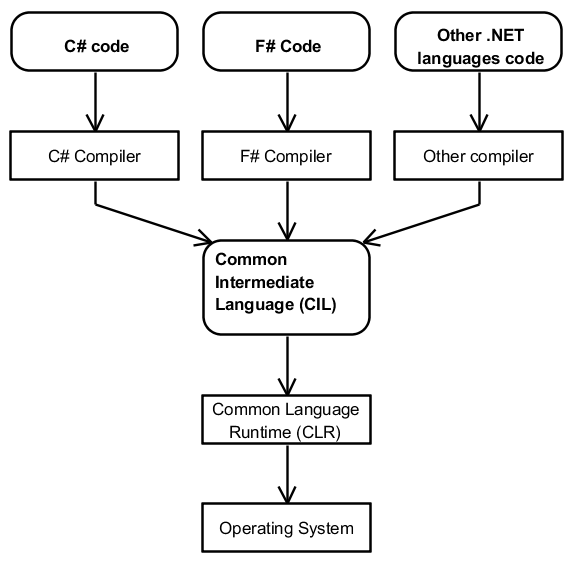
\includegraphics[width=\textwidth]{cli.png}
			\end{column}
		\end{columns}
	\end{frame}

	\begin{frame}
		\frametitle{Зачем так}
		\begin{itemize}
			\item Единый байткод с механизмом оптимизации, интерпретации и генерации машинного кода позволяет экономить время на разработку компиляторов
			\begin{itemize}
				\item Поэтому под .NET можно писать на C\#, F\#, Visual Basic, J\# (зачем бы он ни был нужен), куче сторонних языков (например, Delphi)
			\end{itemize}
			\item Совместимость кода, написанного на разных языках, возможность из кода на F\# без усилий использовать библиотеки на C\# и наоборот
			\item Виртуальная машина знает всё о выполнении программы и многое может проверять (обращения к памяти, границы массивов и т.д.)
			\item JIT-компиляция
			\item Такая схема использовалась для Паскаля и Лиспа аж в 1970-х
		\end{itemize}
	\end{frame}

	\begin{frame}
		\frametitle{Сборка мусора}
		\begin{columns}
			\begin{column}{0.6\textwidth}
				\begin{itemize}
					\item Виртуальная машина сама следит за используемой памятью и освобождает её, когда она перестаёт быть нужной
					\item Корневое множество (глобальные переменные и стек вызовов), достижимое множество
					\item Вызывается, ``когда захочет''
					\item Относительно вычислительно сложно
					\item Устроено обычно довольно хитро
					\begin{itemize}
						\item Поколения, Large Object Heap и т.д.
					\end{itemize}
				\end{itemize}
			\end{column}
			\begin{column}{0.4\textwidth}
				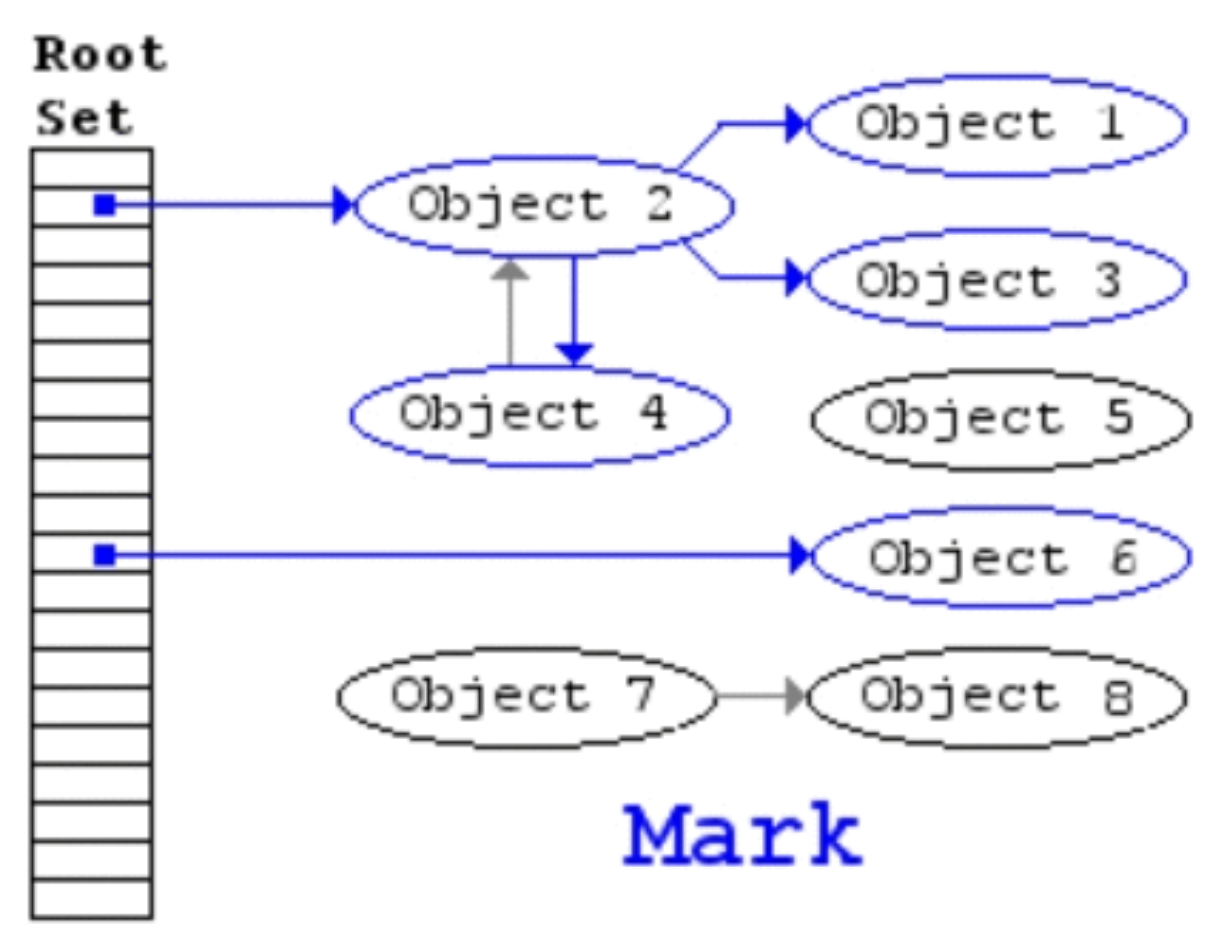
\includegraphics[width=\textwidth]{markAndSweep.png}
			\end{column}
		\end{columns}
	\end{frame}

	\section{Технические детали C\#}

	\begin{frame}[fragile]
		\frametitle{Технические детали C\#}
		\framesubtitle{Как обычно, сначала Hello, world}
		\begin{minted}{csharp}
using System;

namespace HelloWorld
{
    class Program
    {
        static void Main(string[] args)
        {
            Console.WriteLine("Goodbye, cruel world!");
        }
    }
}
		\end{minted}
	\end{frame}

	\begin{frame}[fragile]
		\frametitle{Циклы}
		\begin{minted}{csharp}
for (int i = 0; i < 300; ++i)
{
    Console.WriteLine("Hello, world!");
}
		\end{minted}
		или
		\begin{minted}{csharp}
for (var i = 0; i < 300; ++i)
{
    Console.WriteLine("Hello, world!");
}
		\end{minted}
	\end{frame}

	\begin{frame}[fragile]
		\frametitle{Функции}
		\begin{minted}{csharp}
private static int Factorial(int n)
{
    if (n <= 1)
    {
         return 1;
    }

    return n * Factorial(n - 1);
}
		\end{minted}
		или так:
		\begin{minted}{csharp}
private static int Factorial(int n) 
    => n <= 1 ? 1 : n * Factorial(n - 1);
		\end{minted}
	\end{frame}

	\begin{frame}[fragile]
		\frametitle{Использование}
		\begin{minted}{csharp}
namespace HelloWorld
{
    class Program
    {
        static void Main(string[] args)
        {
            System.Console.WriteLine(Factorial(4));
        }
    }
}
		\end{minted}
	\end{frame}

	\begin{frame}
		\frametitle{Стайлгайд}
		\begin{itemize}
			\item C\# Coding Conventions
			\begin{itemize}
				\item \url{https://docs.microsoft.com/en-us/dotnet/csharp/programming-guide/inside-a-program/coding-conventions}
			\end{itemize}
			\item \url{https://github.com/DotNetAnalyzers/StyleCopAnalyzers}
			\item \href{https://msdn.microsoft.com/en-us/library/3z0aeatx.aspx}{Code Analysis for Managed Code (бывший FxCop)}
			\item Здравый смысл
		\end{itemize}
	\end{frame}

	\begin{frame}
		\frametitle{Элементарные типы}
		\begin{itemize}
			\item Всё --- объект, даже \mintinline{csharp}|int| наследуется от \mintinline{csharp}|Object|
			\item Типы стандартизованы: размер и множество значений одинаковы во всех реализациях
			\item Каждому типу соответствует библиотечный класс
			\begin{itemize}
				\item Например, \mintinline{csharp}|int| --- \mintinline{csharp}|System.Int32|
			\end{itemize}
			\item У каждого типа есть значение по умолчанию
			\begin{itemize}
				\item Им переменные и поля инициализируются при создании
			\end{itemize}
		\end{itemize}
	\end{frame}

	\begin{frame}[fragile]
		\frametitle{Методы у типов}
		\begin{minted}{csharp}
var inputString = Console.ReadLine();
int number = int.Parse(inputString);
		\end{minted}
		--- это то же самое, что
		\begin{minted}{csharp}
var inputString = Console.ReadLine();
int number = Int32.Parse(inputString);
		\end{minted}
	\end{frame}

	\begin{frame}[fragile]
		\frametitle{Массивы}
		\begin{minted}{csharp}
int[] a = new int[10];
		\end{minted}
		или
		\begin{minted}{csharp}
var a = new int[10];
		\end{minted}
		Пример:
		\begin{minted}{csharp}
for (var i = 0; i < a.Length; ++i)
{
    a[i] = i;
}
		\end{minted}
		Двумерные массивы:
		\begin{minted}{csharp}
int[,] numbers = new int[3, 3];
numbers[1, 2] = 2; 
int[,] numbers2 = new int[3, 3] { {2, 3, 2}, {1, 2, 6}, {2, 4, 5} };
		\end{minted}
	\end{frame}

	\begin{frame}[fragile]
		\frametitle{Перечисления}
		Объявление:
		\begin{minted}{csharp}
enum SomeEnum
{
        red,
        green,
        blue
}
		\end{minted}
		Использование:
		\begin{minted}{csharp}
SomeEnum a = SomeEnum.blue;
		\end{minted}
		(ну или через \mintinline{csharp}|var|: \mintinline{csharp}|var a = SomeEnum.blue;|)
	\end{frame}

	\begin{frame}[fragile]
		\frametitle{Структуры}
		\begin{minted}{csharp}
struct Point
{
    public int x;
    public int y;
}
		\end{minted}
	\end{frame}

\end{document}